\section{各画面の説明}
\subsection{ログイン画面}
\subsubsection{画面の概要}
% 画面の概要
この画面は、システムを利用する管理者および学生がログインするためのものです。
図\ref{fig:sc_login}にイメージ図を示します。

\begin{figure}[htbp]
  \begin{center}
    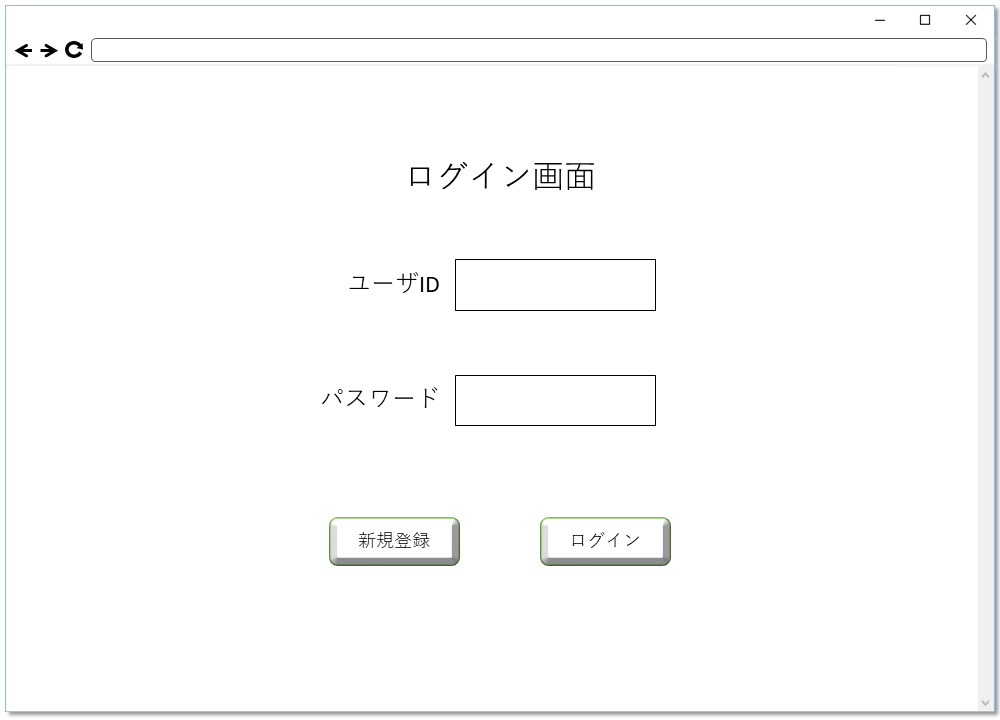
\includegraphics[width=1\linewidth,clip]{./img/sc_login.png}
    \caption{ログイン画面のイメージ図}\label{fig:sc_login}
  \end{center}
\end{figure}

\subsubsection{操作説明}
% 操作説明
ログイン画面での操作説明を以下に示します。
\begin{itemize}
\item アカウントを新規登録する場合
\begin{enumerate}
\item 「新規作成」ボタンを押下すると、「アカウント新規作成画面」に遷移します。
\end{enumerate}
\item ログインする場合
\begin{enumerate}
\item ユーザIDとパスワードを入力します。
\item 「ログイン」ボタンを押下します。
\item ログインが成功すると、管理者アカウントの場合は「授業選択画面」に遷移します。学生アカウントの場合は「授業画面」に遷移します。
      また、ログインが失敗すると、他の画面には遷移しません。
\end{enumerate}
\end{itemize}

\subsection{アカウント新規作成画面}
\subsubsection{画面の概要}
% 画面の概要
この画面は、学生がアカウントを新規作成するためのものです。
図\ref{fig:sc_account_creat}にイメージ図を示します。

\begin{figure}[htbp]
  \begin{center}
    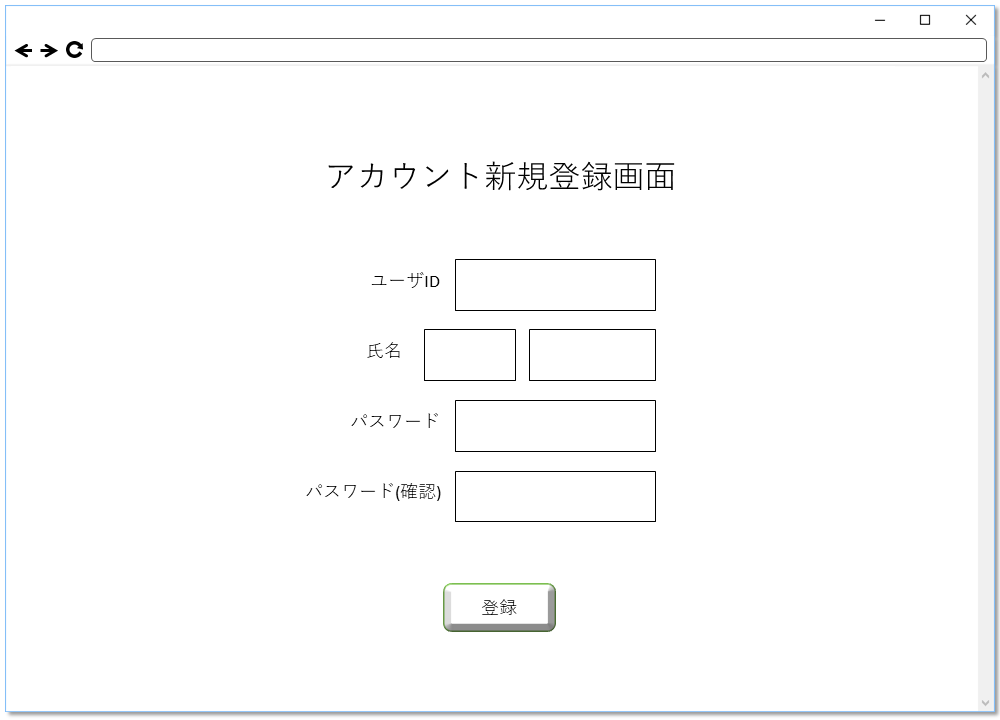
\includegraphics[width=1\linewidth,clip]{./img/sc_account_creat.png}
    \caption{アカウント新規作成画面のイメージ図}\label{fig:sc_account_creat}
  \end{center}
\end{figure}

\subsubsection{操作説明}
% 操作説明
アカウント新規作成画面での操作説明を以下に示します。
\begin{itemize}
\item ユーザID、氏名(フルネーム)およびパスワードを入力します。
なお、パスワードは確認のために2回入力します。
\item 登録ボタンをクリックすると、「ログイン画面」に遷移します。
\end{itemize}

\subsection{管理者用の授業選択画面}
\subsubsection{画面の概要}
% 画面の概要
この画面は、管理者が担当する授業画面へのリンクが表示されています。
また、新規に授業画面を作成することもできます。
図\ref{fig:sc_select_class}にイメージ図を示します。

\begin{figure}[htbp]
  \begin{center}
    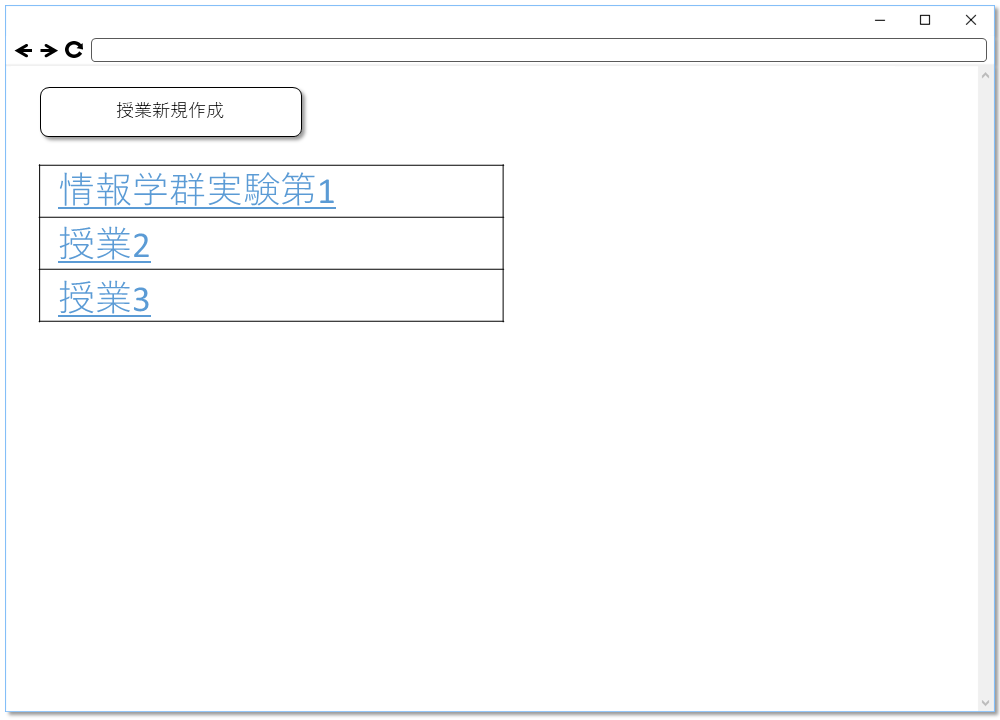
\includegraphics[width=1\linewidth,clip]{./img/sc_select_class.png}
    \caption{管理者用の授業選択画面のイメージ図}\label{fig:sc_select_class}
  \end{center}
\end{figure}

\subsubsection{操作説明}
% 操作説明
管理者用の授業選択画面での操作説明を以下に示します。
\begin{itemize}
\item 「授業新規作成」ボタンを押下すると、「授業カスタマイズ画面」に遷移します。
\item 授業名がその授業画面へのリンクとして表示されているので、そのリンクを押下することで「管理者用の授業画面」に遷移します。
\end{itemize}

\subsection{管理者用の進捗確認画面}
\subsubsection{画面の概要}
% 画面の概要
この画面は、管理者が課題の進捗を確認するためのものです。
図\ref{fig:sc_prog_check}にイメージ図を示します。

\begin{figure}[htbp]
\begin{center}
  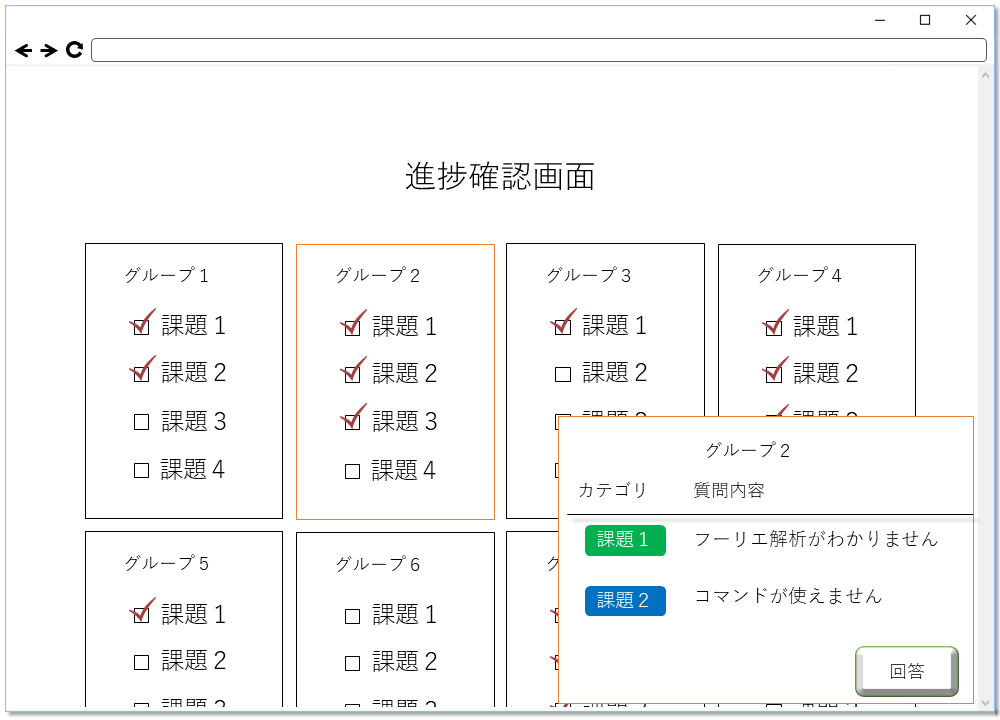
\includegraphics[width=1\linewidth,clip]{./img/sc_prog_check.png}
  \caption{管理者用の授業選択画面のイメージ図}\label{fig:sc_prog_check}
\end{center}
\end{figure}

\subsubsection{操作説明}
% 操作説明
この画面で、各グループの課題の進捗を確認することができます。
また、学生から質問があると、そのグループの枠線が点灯します。
そのグループの枠内をクリックすることで、
画面右下に質問確認のウィンドウが現れます。
そこでは、どの課題で、どのような質問が来たのかを確認することができます。
回答ボタンをクリックすると、質問回答画面へと遷移します。

\subsection{管理者用の回答画面}
\subsubsection{画面の概要}
% 画面の概要
この画面は、管理者が、学生から送信された質問に回答するためのものです。
図\ref{fig:sc_answer}にイメージ図を示します。

\begin{figure}[htbp]
\begin{center}
  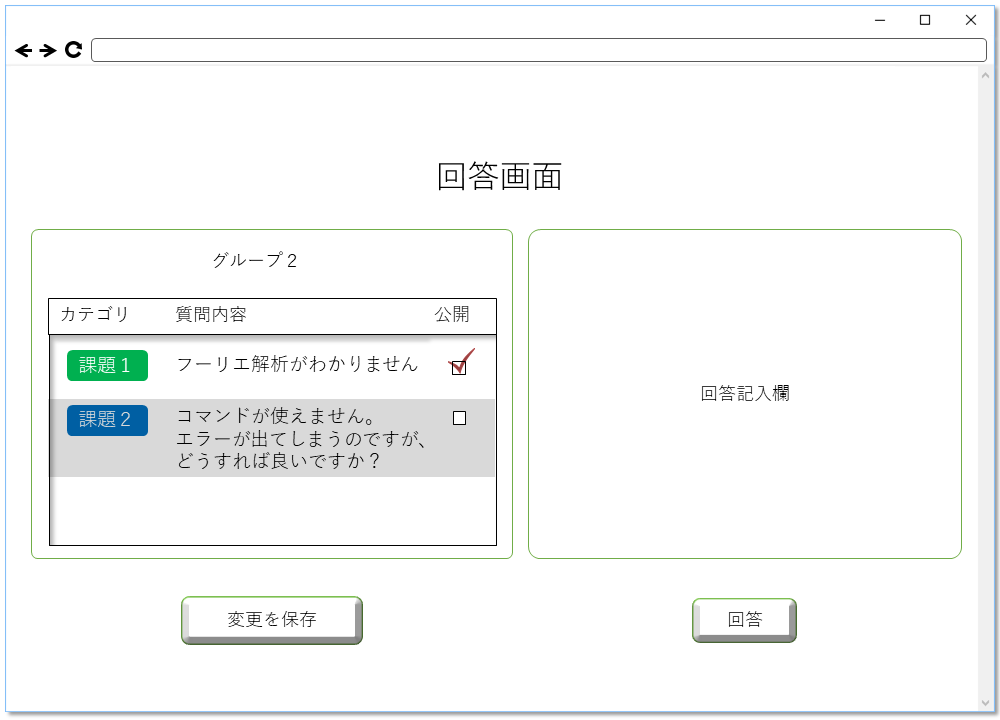
\includegraphics[width=1\linewidth,clip]{./img/sc_answer.png}
  \caption{管理者用の授業選択画面のイメージ図}\label{fig:sc_answer}
\end{center}
\end{figure}

\subsubsection{操作説明}
% 操作説明
質問回答画面には、左側にグループ名とそのグループからの質問が表示されています。
回答をする場合、その質問が表示されている部分を選択し、
右側にある回答記入欄に回答を記入し、回答ボタンをクリックすることで送信します。
質問や回答の内容は他の学生にも閲覧することが可能となっており、
その質問や回答の内容公開するかしないかは、
質問の横にある公開の欄にチェックすることで設定ができます。

\subsection{学生用の授業画面}
\subsubsection{画面の概要}
% 画面の概要
この画面は、学生が受講中の授業の情報を。
図\ref{fig:sc_class_student}にイメージ図を示します。

\begin{figure}[htbp]
\begin{center}
  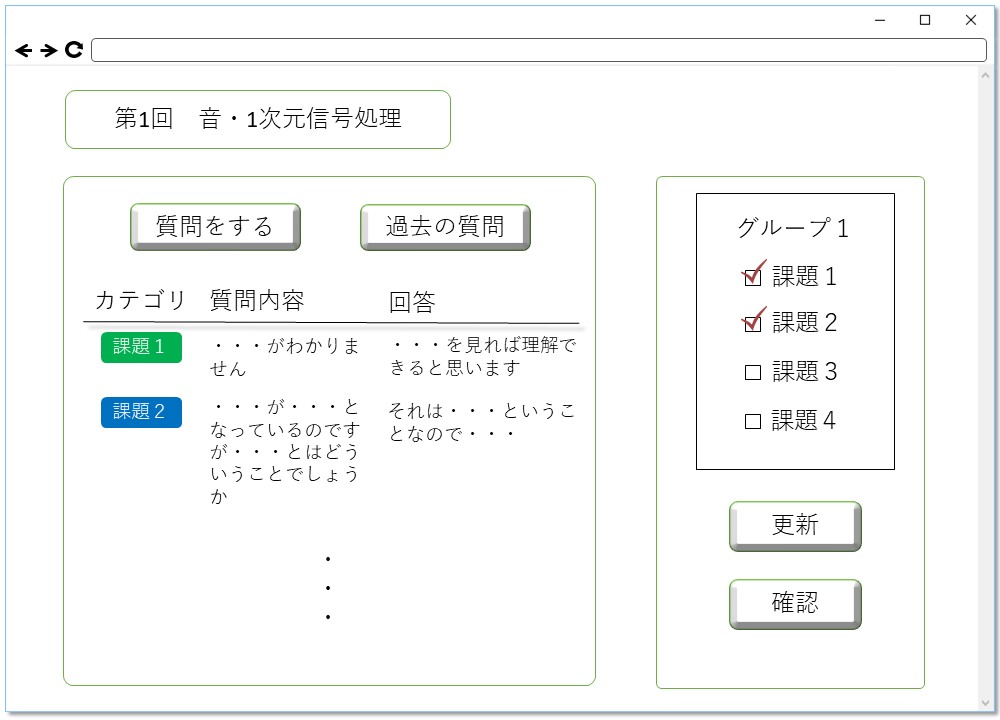
\includegraphics[width=1\linewidth,clip]{./img/sc_class_student.png}
  \caption{学生用の授業画面のイメージ図}\label{fig:sc_class_student}
\end{center}
\end{figure}

\subsubsection{操作説明}
% 操作説明
学生側の授業画面
一番上には今開講されている授業名が表示される
その下の画面左側には質問に関することが、右側には課題の進捗に関することが表示されている

質問に関する画面
画面上部には「質問をする」ボタンと「過去の質問」ボタンがある
「質問をする」ボタンを押すと管理者に質問ができる「質問入力画面」に移動する
「過去の質問」ボタンを押すと今の質問に関する画面が過去の質問を閲覧するための年度選択画面に切り替わる
2つのボタンの下にはその日に出た質問が並んでいる
質問の並びはカテゴリを基準としている

課題の進捗に関する画面
画面上部にある枠では自分のグループ番号と課題ごとのチェックボックスがあり、
その下には課題の進捗状況を更新するボタンと全ての課題が終わった時に管理者
に確認してもらうために呼び出すボタンがある
学生側は課題が終わったと思った時にチェックボックスにチェックを入れ、
更新ボタンを押すことでここまで終わっているということを管理者に知らせることができる

\subsection{質問の年度選択画面}
\subsubsection{画面の概要}
% 画面の概要
この画面は、管理者が。
図\ref{fig:sc_select_year}にイメージ図を示します。

\begin{figure}[htbp]
\begin{center}
  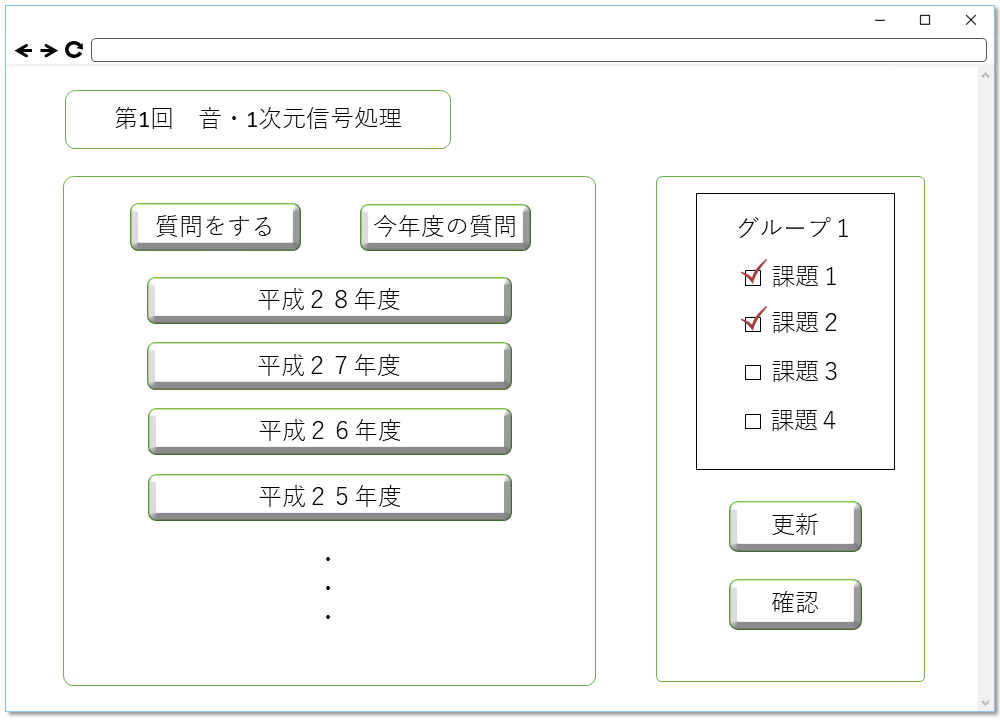
\includegraphics[width=1\linewidth,clip]{./img/sc_select_year.png}
  \caption{質問の年度選択画面のイメージ図}\label{fig:sc_select_year}
\end{center}
\end{figure}

\subsubsection{操作説明}
% 操作説明
画面上部には「質問をする」ボタンと、「今年度の質問」ボタンがある
「質問をする」ボタンは「学生側の授業画面」と同じ機能を持つ
「今年度の質問」ボタンを押すと今年度の質問が表示されている「学生側の授業画面」に戻る
上の2つのボタンの下に並んでいる年度ボタンを押すことでその年度の質問画面に切り替わる
各年度の質問画面は今年度の質問が書いてあるところと同じ画面で質問の内容がその年度のものになっている

\subsection{授業内容画面}
\subsubsection{画面の概要}
% 画面の概要
この画面は、管理者が。
図\ref{fig:sc_class_content}にイメージ図を示します。

\begin{figure}[htbp]
\begin{center}
  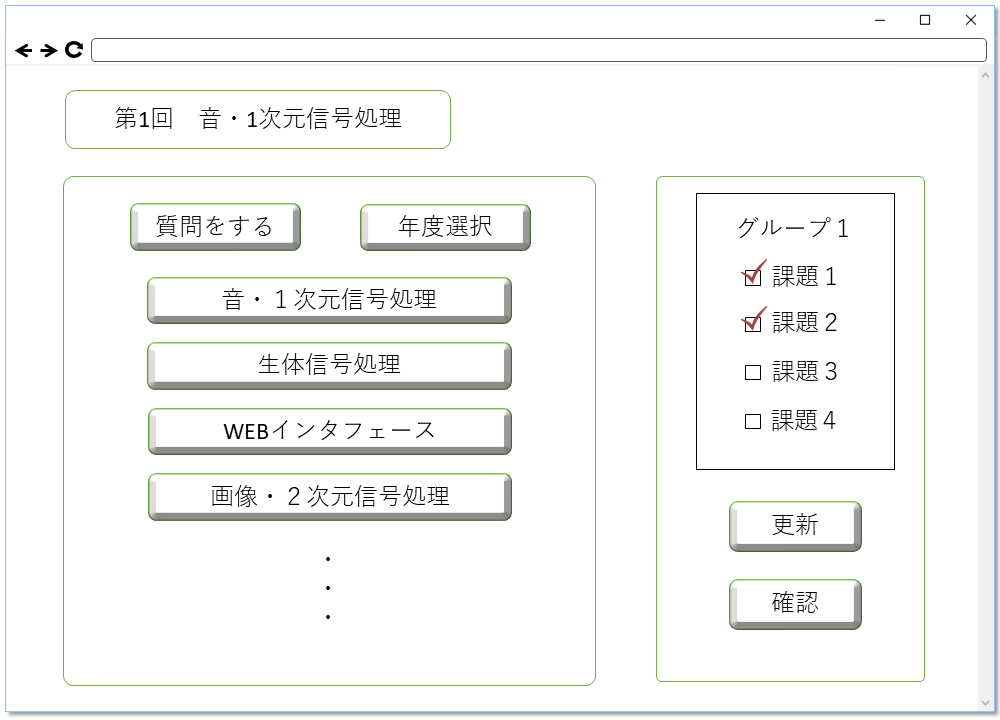
\includegraphics[width=1\linewidth,clip]{./img/sc_class_content.png}
  \caption{授業内容画面のイメージ図}\label{fig:sc_class_content}
\end{center}
\end{figure}

\subsubsection{操作説明}
% 操作説明
画面上部には「質問をする」ボタンと、「今年度の質問」ボタンがある
「質問をする」ボタンは「学生側の授業画面」と同じ機能を持つ
「今年度の質問」ボタンを押すと今年度の質問が表示されている「学生側の授業画面」に戻る
上の2つのボタンの下に並んでいる年度ボタンを押すことでその年度の質問画面に切り替わる
各年度の質問画面は今年度の質問が書いてあるところと同じ画面で質問の内容がその年度のものになっている

\subsection{過去質問画面}
\subsubsection{画面の概要}
% 画面の概要
この画面は、学生が。
図\ref{fig:sc_pre_q}にイメージ図を示します。

\begin{figure}[htbp]
\begin{center}
  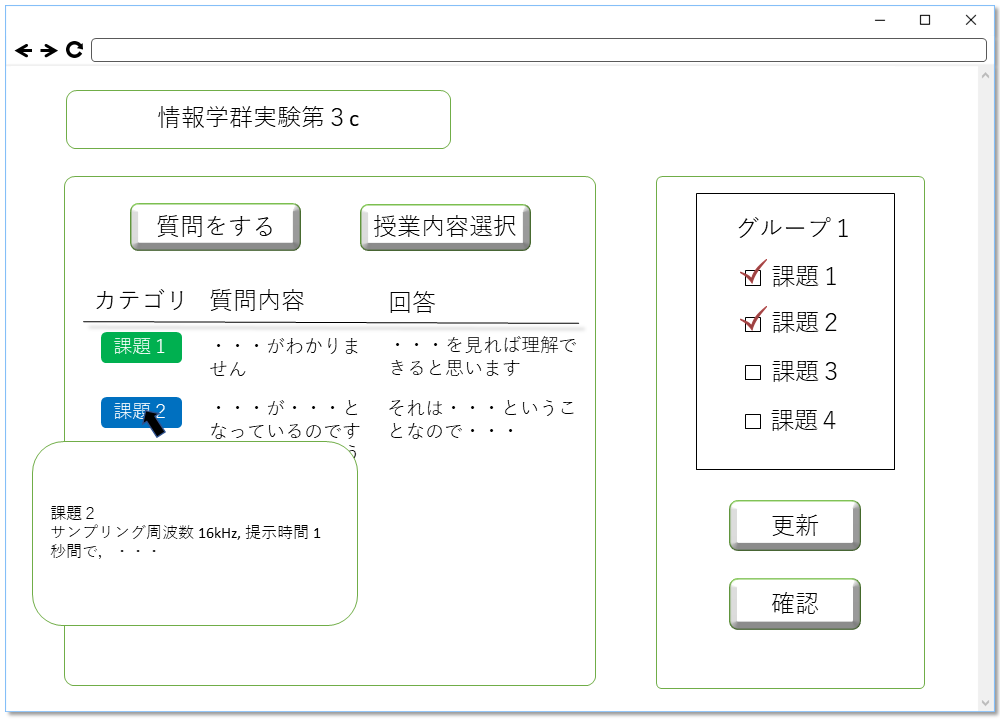
\includegraphics[width=1\linewidth,clip]{./img/sc_pre_q.png}
  \caption{過去質問画面のイメージ図}\label{fig:sc_pre_q}
\end{center}
\end{figure}

\subsubsection{操作説明}
% 操作説明
「質問をする」ボタンを押すと他の画面同様「質問入力画面」に移動
「授業内容選択」ボタンを押すと「授業内容画面」に戻る
2つのボタンの下には選択した授業内容について過去に出た質問が表示される
カテゴリの「課題1」や「課題2」にカーソルを合わせるとそのカテゴリの課題内容が表示される

\subsection{質問入力画面}
\subsubsection{画面の概要}
% 画面の概要
この画面は、学生が。
図\ref{fig:sc_input_q}にイメージ図を示します。

\begin{figure}[htbp]
\begin{center}
  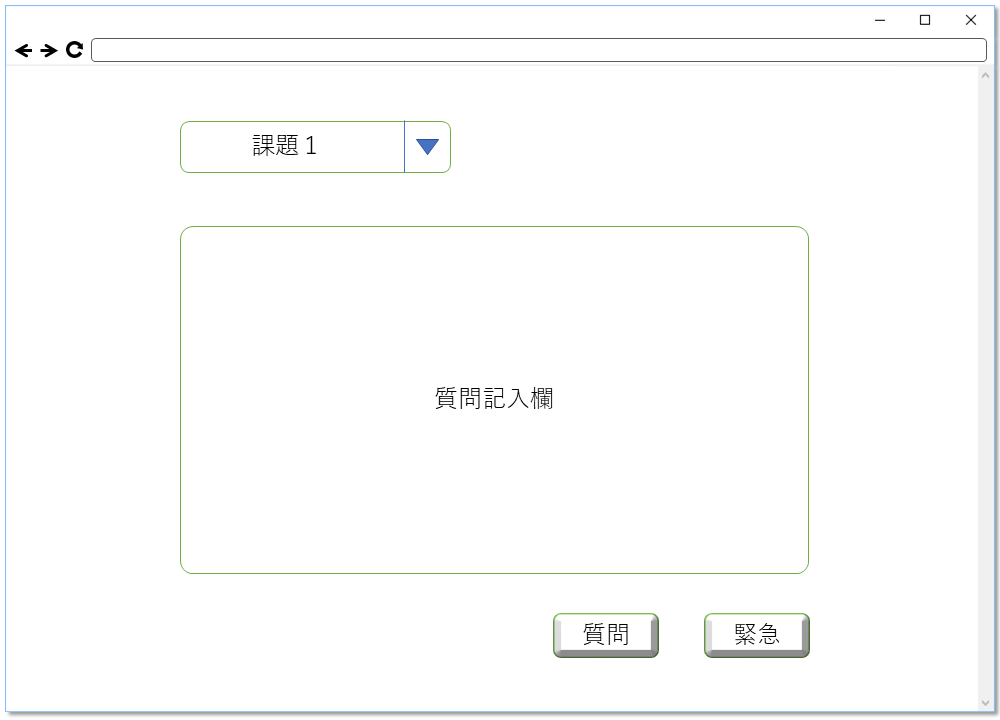
\includegraphics[width=1\linewidth,clip]{./img/sc_input_q.png}
  \caption{質問入力画面のイメージ図}\label{fig:sc_input_q}
\end{center}
\end{figure}

\subsubsection{操作説明}
% 操作説明
この画面での質問の手順を示す
まず画面上部の枠からどの課題に対して質問をするのかを選択する
次にその下の欄に質問内容を記入し、質問記入欄の下にある質問ボタン
を押すことで管理者に質問を送信することができる
課題に対する質問ではなくそれ以外で問題が起こって課題が
進められない場合などは課題選択欄の最後にある「その他」を選択して内容を記入し、
質問ボタンの横にある緊急ボタンを押すと、質問とは別の緊急案件として
管理者に報告することができる

\subsection{授業詳細設定画面}
\subsubsection{画面の概要}
% 画面の概要
この画面は、学生が。
図\ref{fig:sc_class_detail1}、\ref{fig:sc_class_detail2}にイメージ図を示します。

\begin{figure}[htbp]
\begin{center}
  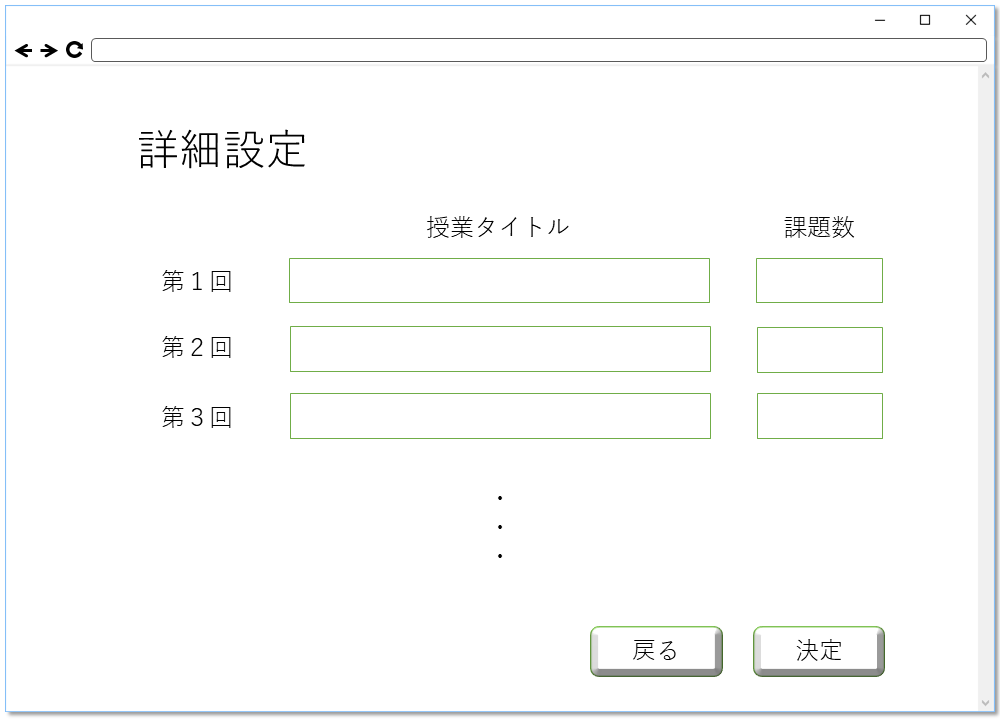
\includegraphics[width=1\linewidth,clip]{./img/sc_class_detail1.png}
  \caption{授業詳細設定画面のイメージ図1}\label{fig:sc_class_detail1}
\end{center}
\end{figure}

\begin{figure}[htbp]
\begin{center}
  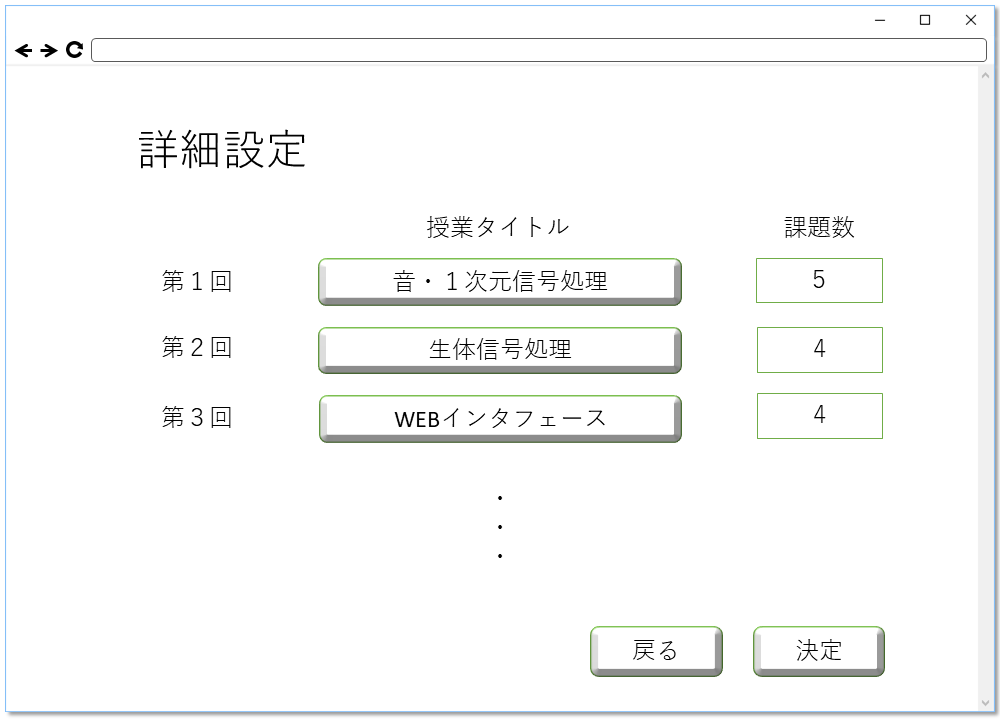
\includegraphics[width=1\linewidth,clip]{./img/sc_class_detail2.png}
  \caption{授業詳細設定画面のイメージ図2}\label{fig:sc_class_detail2}
\end{center}
\end{figure}

\subsubsection{操作説明}
% 操作説明
詳細設定画面1
この画面は「新規作成画面」で入力した授業回数に応じてそれぞれの回の授業タイトルと課題数を入力する画面
授業タイトルには学生側が過去の質問を見ようとした時でもわかるようなタイトルを入力
課題数にはその回に出る課題の数を入力
全て入力して終わったら決定ボタンで「詳細設定画面2」に移動する
戻るボタンで「新規作成画面」に戻る
詳細設定画面2
この画面は「詳細設定画面1」で入力したタイトルとその課題数に応じて課題の内容を入力する画面に移動する前の画面
授業タイトルボタンを押すことでそのタイトルの課題内容を入力する「詳細設定画面3」に移動
全てのタイトルに応じた授業内容を入力し終わったら、決定ボタンを押すことで

\subsection{管理者用の進捗確認画面}
\subsubsection{画面の概要}
% 画面の概要
この画面は、。
図\ref{fig:sc_prog_check_one1}、\ref{fig:sc_prog_check_one2}にイメージ図を示します。

\begin{figure}[htbp]
\begin{center}
  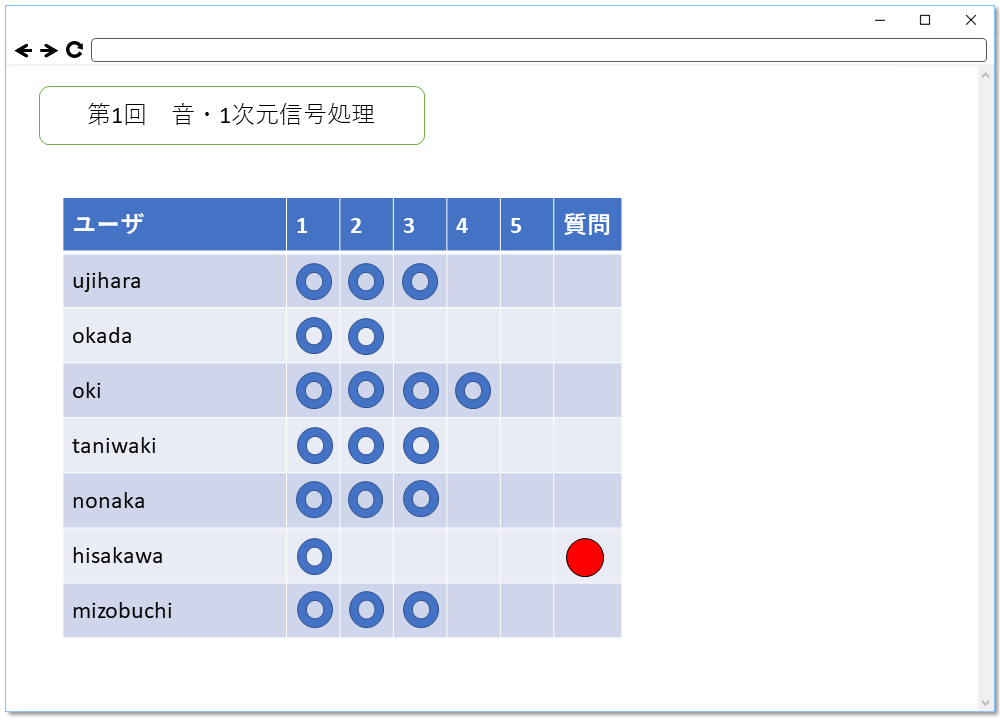
\includegraphics[width=1\linewidth,clip]{./img/sc_prog_check_one1.png}
  \caption{管理者用の進捗確認画面のイメージ図1}\label{fig:sc_prog_check_one1}
\end{center}
\end{figure}

\begin{figure}[htbp]
\begin{center}
  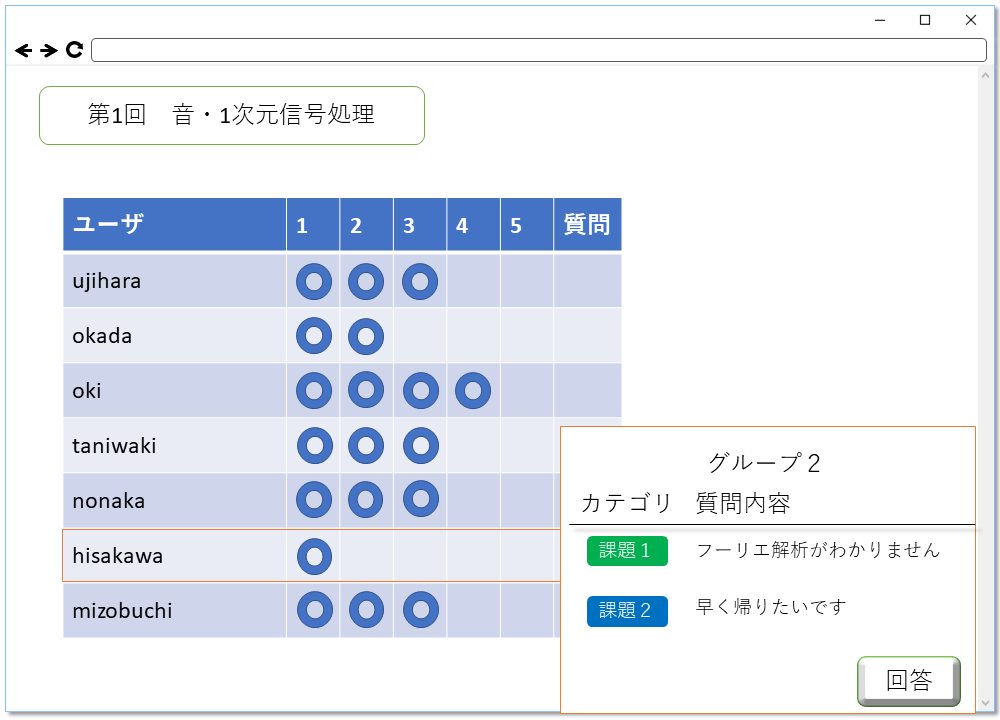
\includegraphics[width=1\linewidth,clip]{./img/sc_prog_check_one2.png}
  \caption{管理者用の進捗確認画面のイメージ図2}\label{fig:sc_prog_check_one2}
\end{center}
\end{figure}

\subsubsection{操作説明}
% 操作説明

\subsection{授業画面作成画面}
\subsubsection{画面の概要}
% 画面の概要
この画面は、。
図\ref{fig:sc_class_creat1}、\ref{fig:sc_class_creat2}にイメージ図を示します。

\begin{figure}[htbp]
\begin{center}
  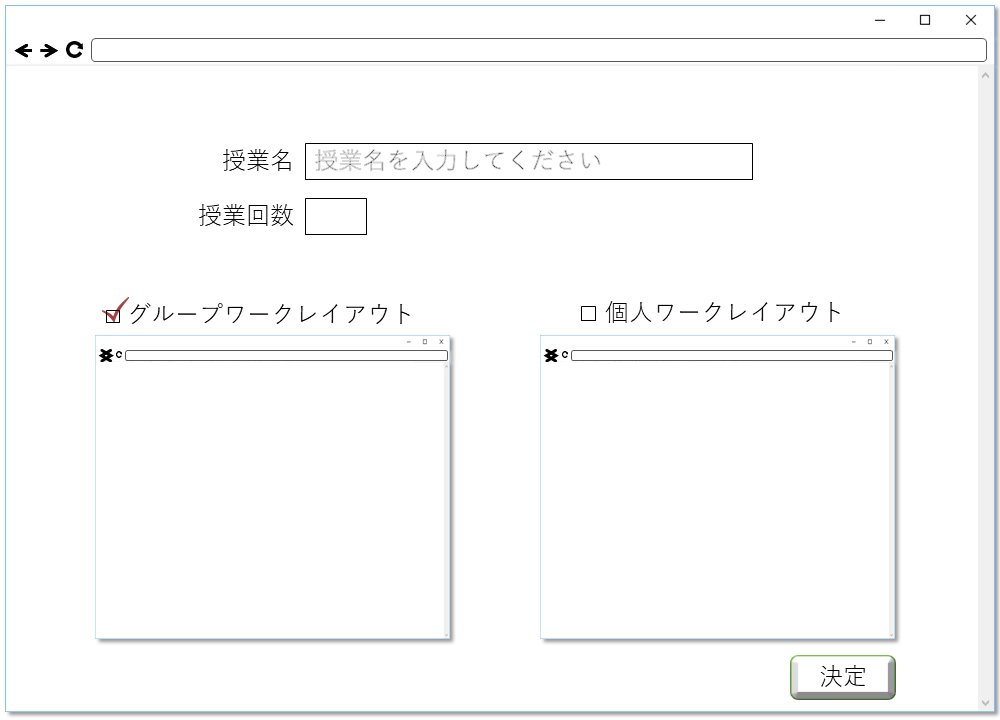
\includegraphics[width=1\linewidth,clip]{./img/sc_class_creat1.png}
  \caption{授業画面作成画面のイメージ図1}\label{fig:sc_class_creat1}
\end{center}
\end{figure}

\begin{figure}[htbp]
\begin{center}
  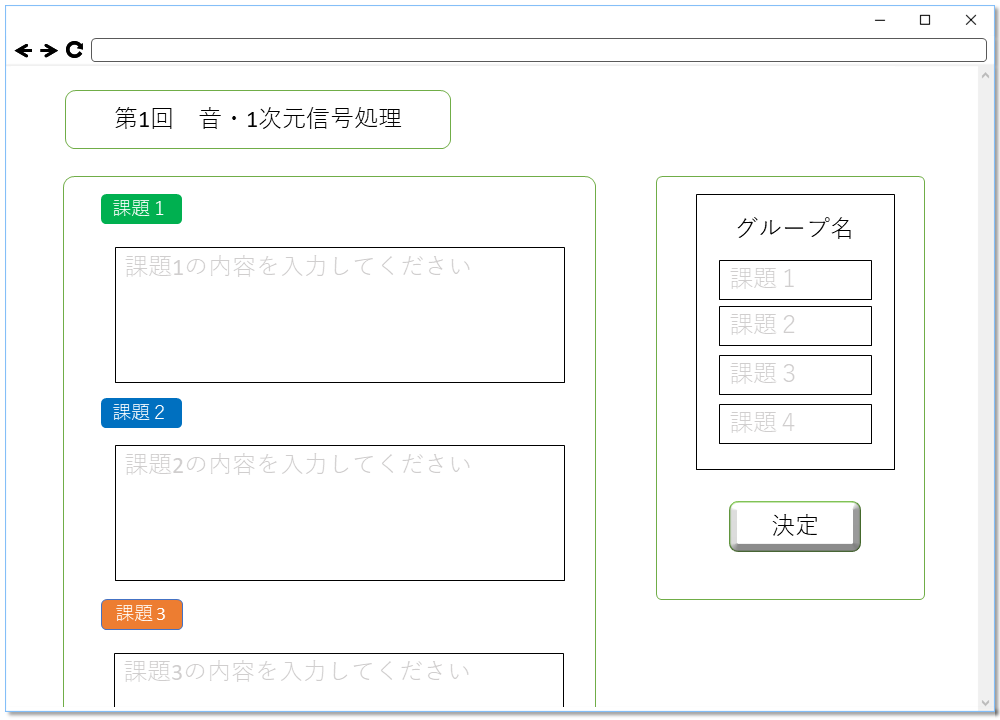
\includegraphics[width=1\linewidth,clip]{./img/sc_class_creat2.png}
  \caption{授業画面作成画面のイメージ図2}\label{fig:sc_class_creat2}
\end{center}
\end{figure}
